\section*{Theoretical Framework}

We now build the mathematical scaffold that explains the three motivating facts
and delimits exactly what any post-training recipe can and cannot achieve. The
development is deliberately conservative: we state what holds as an \emph{identity},
label empirical regularities as such, and---crucially---prove a
\emph{negative} result that overturns an appealing but false ``ceiling''
conjecture and thereby opens the design space our methodology occupies. Every
theoretical claim is paired with the experimental evidence that tests it
(Table~\ref{tab:ledger}).

\subsection*{Setup and definitions}

A policy $\pi_\theta(y\mid x)$ generates a solution $y$ to a problem $x$. A
\textbf{verifier} $V(x,y)\in\{0,1\}$ is \emph{parameter-independent}: an executor
or exact-match checker that does not depend on $\theta$ \textbf{(A1)}. Define the
per-prompt \textbf{success mass} and the population objective (single-attempt
reliability),
\[
p_\theta(x)=\mathbb{E}_{y\sim\pi_\theta(\cdot\mid x)}[V(x,y)],
\qquad
J(\theta)=\mathbb{E}_{x\sim\mathcal{D}}[p_\theta(x)]=\text{pass}@1,
\]
and coverage $\;\mathrm{cov}_k(\theta)=\mathbb{E}_x\!\big[1-(1-p_\theta(x))^{k}\big]$.
Write $\mathcal{C}(x)=\{y:V(x,y)=1\}$ (verified-correct) and $\mathcal{I}(x)$
(verified-incorrect). From a base checkpoint $\theta_0$ define \textbf{headroom}
$h(x)=1-p_{\theta_0}(x)$ and, at sampling budget $C$, \textbf{accessibility}
$a(x;C)=1-(1-p_{\theta_0}(x))^{C}$. For a self-generated pair
$(y^{+}\!\in\!\mathcal{C},\,y^{-}\!\in\!\mathcal{I})$ the \textbf{logit margin} is
$m_\theta(x)=\log\pi_\theta(y^{+}\!\mid x)-\log\pi_\theta(y^{-}\!\mid x)$. Three
operators are trained from the shared $\theta_0$: \emph{GRPO} (on-policy
policy-gradient on $V$), \emph{RFT} (multi-epoch cross-entropy on a verified bank
$B=\{(x,y):V=1\}$ sampled from $\pi_{\theta_0}$), and \emph{VSF} (GRPO plus a
persistent prompt-balanced replay floor over $B$, used as a causal probe).

\subsection*{3.1 The gradient-family identity: why on-policy reward acquires little}

\paragraph{Theorem 1 (Gradient-family identity).}
Under (A1), for every prompt $x$,
\begin{equation}
\nabla_\theta\,p_\theta(x)=p_\theta(x)\;
\mathbb{E}_{y\sim\pi_\theta(\cdot\mid x)}\!\big[\nabla_\theta\log\pi_\theta(y\mid x)\mid V(x,y)=1\big].
\label{eq:identity}
\end{equation}
Consequently (i) the within-prompt-normalised RFT gradient on current-policy
successes equals $\nabla_\theta\log p_\theta(x)$, and (ii) the binary-reward policy
gradient equals $p_\theta(x)$ times the \emph{same} direction. RFT and outcome-RL
are therefore \emph{not distinct gradient families}; they differ only by a positive
per-prompt scalar and by which prompts carry a nonzero success-gradient.

\emph{Proof.} Score-function identity $\nabla_\theta p_\theta(x)=\mathbb{E}[V\nabla\log\pi]$;
condition on $V=1$ (the $V=0$ term vanishes as $V\in\{0,1\}$) and normalise by
$p_\theta(x)=\Pr(V{=}1)$. The policy gradient of $\mathbb{E}[V]$ is
$\mathbb{E}[V\nabla\log\pi]=p_\theta(x)\cdot(\text{that conditional mean})$. $\square$

\paragraph{Corollary 1.1 (coverage throttling).}
Because the on-policy update weights each prompt's success-gradient by
$p_\theta(x)$, a prompt the base model almost never solves ($p_{\theta_0}(x)\!\approx\!0$)
receives $\approx\!0$ update: outcome-RL cannot acquire base-failed prompts. RFT's
\emph{decoupled} multi-epoch replay over $B$ supplies those gradients regardless
of current success mass. This predicts GRPO $\text{pass}@1\!\approx\!$ base while
RFT acquires broadly.

The prediction is confirmed twice over. Numerically, the turnover-robust
population acquisition of GRPO is $A=0.010$ (net $+0.001$) versus RFT $A=0.132$
(net $+0.126$) on the same cell (Table~\ref{tab:alphabeta}). Distributionally,
GRPO leaves the per-prompt reliability histogram identical to the base model---%
$79\%$ of prompts remain in the ``almost never solved'' pile
($\hat p<0.1$)---while RFT rescues a third of them (Fig.~\ref{fig:reldist}).

\emph{Scope (honest).} Eq.~\eqref{eq:identity} is an exact per-prompt identity for
current-policy expectations. A stale multi-epoch bank, clipped/group-normalised
GRPO, and cross-prompt reweighting each perturb the aggregate direction; we do
\emph{not} claim ``all RFT--GRPO gaps are procedural'' in general---only the
identity and the coverage-throttling mechanism it exposes.

\subsection*{3.2 Positive-only replay is mode-covering: the selection axis is untouched}

\paragraph{Theorem 2 (support-boundedness, scoped).}
Under (A1), the verified-only cross-entropy objective contributes \emph{zero
example-specific gradient} on any prompt absent from the bank; any change there is
transfer through shared parameters. (We state this as an identity about the
example-specific term, not as an upper bound on out-of-distribution improvement:
shared-parameter updates \emph{can} move off-support predictions, so no
generalisation ceiling is claimed.)

\paragraph{Proposition 1 (no margin control).}
The RFT gradient $\nabla_\theta \sum_{y\in\mathcal{C}(x)}\log\pi_\theta(y\mid x)$
contains no term that \emph{decreases} $\log\pi_\theta(y^{-}\mid x)$ for a
verified-incorrect $y^{-}$; it therefore does not directly increase the margin
$m_\theta(x)$. Positive-only imitation is \emph{mode-covering}: it can raise the
probability of correct completions without suppressing the incorrect ones the
model also samples.

This is the mechanistic origin of the reliability gap (Motivation \S2). On the
same held-out verified pairs, RFT raises $\log\pi(y^{+})$ from $-0.110$ to
$-0.092$ but raises $\log\pi(y^{-})$ almost identically ($-0.139\!\to\!-0.119$),
leaving the margin flat ($0.029\!\to\!0.027$); GRPO moves neither
(Motivation Table~3, Fig.~3). Coverage rises, single-attempt \emph{selection} does
not.

\subsection*{3.3 Accessibility gating: gains are non-monotone in difficulty}

Combining Thm.~1--2, the realised new-coverage gain on the reachable frontier
behaves as $G(x)\approx h(x)\,a(x;C)\,\tau(x)$ for a prompt-wise transfer
coefficient $\tau(x)\in[0,1]$. Treating headroom $h$ as the free variable suggests
a \emph{posited} closed form
\begin{equation}
G(h)=\tau\,h\,(1-h^{C}),\qquad
h^{\star}=\Big(\tfrac{1}{C+1}\Big)^{1/C},
\label{eq:invU}
\end{equation}
which is non-monotone ($G(0)=G(1)=0$, single interior maximum). Empirically the
RFT gain does rise then fall in headroom, and regression $\beta$ (probability a
base-correct prompt becomes wrong, coverage level) \emph{grows} monotonically with
difficulty as usable signal per prompt vanishes: $\beta_{\text{GRPO}}=0.278,0.370,
0.472$ across mid/hard/vhard (Fig.~\ref{fig:beta}).

\paragraph{Empirical Regularity 1 (stated honestly, not as a law).}
Eq.~\eqref{eq:invU} is a \emph{posited} gain model, not derived from the training
dynamics. Its predicted peak $h^{\star}\!\in\![0.76,0.90]$ (for $C{=}8\text{--}32$)
does \emph{not} match the observed peak ($\approx\!0.6$), and the empirical curve
pools model size with difficulty, so it is not a causal law. We therefore report
the inverted-U only as a pooled empirical shape: gain is bounded by headroom from
above yet collapses when accessibility $a(x;C)\!\to\!0$. Reachability is not
reliability---and neither is it free at the extremes.

\subsection*{3.4 No universal ceiling: CE-optimality $\neq$ accuracy-optimality}

An earlier version of this theory conjectured that once the accessible bank is
saturated, \emph{no} wrapper can exceed RFT---i.e.\ RFT is a universal ceiling. We
\textbf{retract} that conjecture: it conflated sharing a gradient span
(Thm.~1) with sharing an optimum. The following counterexample, which we verified
analytically, shows the RFT fixed point can be strictly suboptimal in accuracy on
the very same support.

\paragraph{Theorem 3 (no ceiling).}
There exist verified-training instances in which the multi-epoch RFT fixed point
(the prompt-balanced cross-entropy optimum on the bank) does \emph{not} maximise
$J(\theta)$, even with shared support and a scalar parameter. Concretely, take two
equal-weight prompts and $\theta\in(0,1)$ with $p_1(\theta)=\theta$,
$p_2(\theta)=1-\tfrac34\theta$. The prompt-balanced bank cross-entropy
$\mathrm{CE}(\theta)=-\tfrac12[\log\theta+\log(1-\tfrac34\theta)]$ has its unique
minimiser at $\theta^{\star}=\tfrac23$, whereas the mean accuracy
$J(\theta)=\tfrac12+\tfrac18\theta$ is strictly increasing. Hence
\[
J(\theta^{\star})=0.583 \;<\; J(0.9)=0.613 .
\]
RFT converges to the CE optimum ($\theta=\tfrac23$) yet a higher-accuracy solution
($\theta>\tfrac23$) exists on the same support (Fig.~\ref{fig:counterexample}).

\emph{Consequence.} An objective that is directed at \emph{accuracy/selection}
rather than at bank likelihood can, in principle, exceed RFT. The failed
ceiling conjecture is not a liability---it is the theoretical licence for a new
method. Combined with Prop.~1 (RFT does not control the margin) and Cor.~1.1
(GRPO cannot reach base-failed prompts), the open lever is precisely the margin
$m_\theta(x)$.

\subsection*{3.5 The selection principle (foundation of the methodology)}

\paragraph{Proposition 2 (margin $\Rightarrow$ reliability).}
Restrict attention to a covered prompt whose reachable set is dominated by one
correct mode $y^{+}$ and one incorrect mode $y^{-}$ (the empirically relevant
regime after RFT, where coverage is high). With logits $s^{+},s^{-}$ and
$p_\theta(x)=\sigma\!\big(m_\theta(x)+c(x)\big)$ for a prompt constant $c(x)$ and
the logistic $\sigma$, the single-attempt success mass is \emph{strictly
increasing in the margin} $m_\theta(x)$:
\[
\frac{\partial\, p_\theta(x)}{\partial\, m_\theta(x)}
=\sigma'\!\big(m_\theta(x)+c(x)\big)>0 .
\]
Thus an objective that raises $m_\theta(x)$ on covered prompts increases
$\text{pass}@1$ \emph{without expanding the support} (coverage held fixed)---it
acts on selection, the axis positive-only CE leaves flat (Prop.~1) and on-policy
reward cannot reach (Cor.~1.1), and which Thm.~3 shows no ceiling forbids.

This proposition is the pivot to our methodology: a \emph{decoupled,
verified-preference} objective trained on the model's own
$(y^{+}\!,y^{-})$ pairs increases $m_\theta$ by \emph{suppressing} the
verified-incorrect mode, reallocating probability mass
$\mathcal{I}\!\to\!\mathcal{C}$. We develop and test it in the next section; its
predicted signature (margin up via $\log\pi(y^{-})$ down, $\text{pass}@1$ up at
constant coverage) is the last row of Table~\ref{tab:ledger}.

\subsection*{3.6 Measurement rigor: net accuracy hides a bimodal process}

A recurring failure mode in this literature is reporting \emph{net} accuracy or
\emph{coverage}, both of which mislead. We decompose every comparison per problem
into acquisition $A=\mathbb{E}_x[(p_{\text{arm}}(x)-p_{\text{base}}(x))_{+}]$ and
regression $D=\mathbb{E}_x[(p_{\text{base}}(x)-p_{\text{arm}}(x))_{+}]$ on the
single-attempt estimate $\hat p=c/k$, and calibrate against a \emph{null} obtained
from two independent evaluation passes of the \emph{unchanged} checkpoint
(sampling turnover with zero training). Table~\ref{tab:alphabeta} shows the
consequences: GRPO's flat net accuracy hides essentially no learning
($A=0.010$), RFT's gain is genuine acquisition ($A=0.132$) with negligible true
regression ($D=0.006$), and the large ``forgetting'' suggested by a naive
coverage-level accounting ($\text{null}\,\beta\!\approx\!0.5$) is almost entirely
sampling turnover. The prescription we adopt throughout: \emph{report
$(\text{pass}@1,A,D)$ against the unchanged-checkpoint null, not net
$\Delta$accuracy or coverage.}

\begin{table}[htbp]
\centering
\caption{Turnover-robust acquisition/regression decomposition (comp, Coder-3B,
$n{=}200$, $k{=}16$). ``null'' columns are the acquire/regress expected from
sampling turnover of the \emph{unchanged} checkpoint (zero training). GRPO's net
$+0.001$ reflects no real acquisition; RFT's $+0.126$ is genuine acquisition with
near-zero true regression. The naive coverage-level regression ($\text{null}\,D$)
is a turnover artefact, not forgetting.}
\label{tab:alphabeta}
\begin{tabular}{lccccccc}
\toprule
Arm & $\text{pass}@1$ & $\mathrm{cov}_{16}$ & null $A$ & null $D$ & $A$ (acq.) & $D$ (reg.) & net$@1$ \\
\midrule
base & 0.090 & 0.330 & --    & --    & --    & --    & --      \\
GRPO & 0.091 & 0.353 & 0.055 & 0.549 & 0.010 & 0.009 & $+0.001$ \\
RFT  & 0.216 & 0.610 & 0.129 & 0.467 & \textbf{0.132} & 0.006 & $\mathbf{+0.126}$ \\
VSF  & 0.128 & 0.470 & 0.071 & 0.485 & 0.044 & 0.007 & $+0.037$ \\
\bottomrule
\end{tabular}
\end{table}

\subsection*{Summary: what is proven, what is empirical, what is retracted}

\begin{table}[htbp]
\centering
\caption{The theory--evidence ledger. Each claim is tagged by epistemic status.
The one retraction (Thm.~3) is the pivot that licenses the methodology; the final
row is the prediction the method is designed to satisfy and which the next section
confirms.}
\label{tab:ledger}
\begin{tabular}{p{4.0cm}p{4.3cm}p{3.1cm}p{2.0cm}}
\toprule
Theoretical claim & Testable prediction & Evidence & Status \\
\midrule
Thm.~1 identity + Cor.~1.1 coverage throttling &
GRPO acquires $\approx\!0$ on base-failed prompts; RFT $\gg$ GRPO at $\text{pass}@1$ &
$A$: GRPO $0.010$ vs RFT $0.132$; GRPO $79\%$ stuck (Fig.~\ref{fig:reldist}) &
\textbf{Confirmed} \\
Prop.~1 mode-covering &
RFT lifts $\log\pi(y^{+})$ \emph{and} $\log\pi(y^{-})$; margin flat &
$0.029\!\to\!0.027$ (Motiv.\ Tab.~3) &
\textbf{Confirmed} \\
Emp.~Reg.~1 accessibility gating &
gain non-monotone in headroom; $\beta$ grows with difficulty &
$\beta_{\text{G}}{:}\,.28/.37/.47$ (Fig.~\ref{fig:beta}) &
\emph{Emp.} (pooled) \\
Thm.~3 no ceiling &
$\exists$ instance: CE-opt.\ $<$ accuracy-opt.\ &
$J(\tfrac23){=}.583 < J(.9){=}.613$ (Fig.~\ref{fig:counterexample}) &
\textbf{Proven} (retracts prior ceiling) \\
Prop.~2 selection &
$\uparrow$ margin (via $\downarrow\log\pi(y^{-})$) $\Rightarrow$ $\uparrow\text{pass}@1$, coverage flat &
tested in Methodology &
Predicted $\rightarrow$ verified \\
\bottomrule
\end{tabular}
\end{table}

\begin{figure}[htbp]
\centering
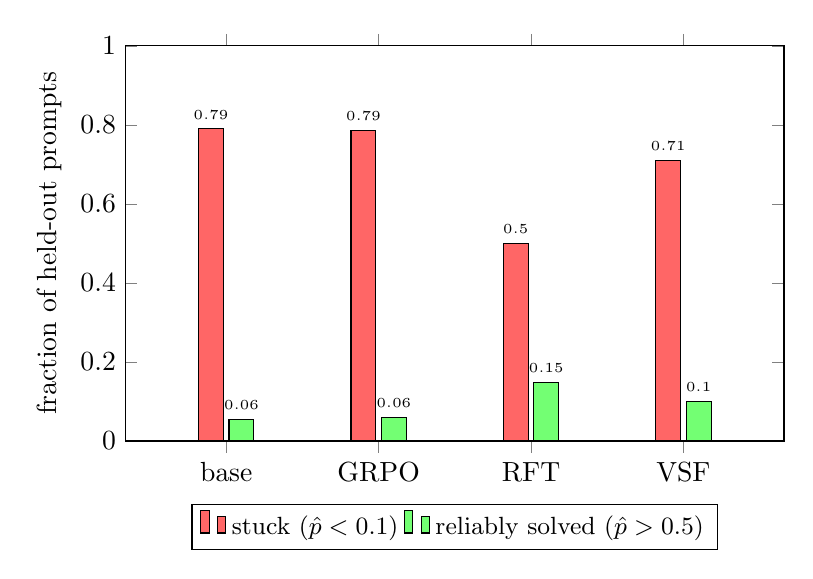
\begin{tikzpicture}
\begin{axis}[
  width=0.82\textwidth, height=6.6cm,
  ybar, bar width=9pt,
  ymin=0, ymax=1.0,
  ylabel={fraction of held-out prompts},
  symbolic x coords={base, GRPO, RFT, VSF},
  xtick=data,
  legend style={at={(0.5,-0.16)},anchor=north,legend columns=2,font=\small},
  enlarge x limits=0.22,
  nodes near coords, nodes near coords style={font=\tiny},
  every node near coord/.append style={/pgf/number format/fixed,/pgf/number format/precision=2},
]
\addplot[fill=red!60] coordinates {(base,0.790) (GRPO,0.785) (RFT,0.500) (VSF,0.710)};
\addplot[fill=green!55] coordinates {(base,0.055) (GRPO,0.060) (RFT,0.148) (VSF,0.100)};
\legend{stuck ($\hat p<0.1$), reliably solved ($\hat p>0.5$)}
\end{axis}
\end{tikzpicture}
\caption{Per-prompt reliability distribution (comp, Coder-3B, $n{=}200$). GRPO is
indistinguishable from base---it rescues \emph{none} of the $79\%$ stuck prompts,
the distributional signature of coverage throttling (Cor.~1.1). RFT moves a third
out of the stuck pile via broad verified replay, but a large stuck mass remains,
because positive-only replay cannot suppress incorrect modes (Prop.~1).}
\label{fig:reldist}
\end{figure}

\begin{figure}[htbp]
\centering
\begin{tikzpicture}
\begin{axis}[
  width=0.78\textwidth, height=6.8cm,
  xlabel={parameter $\theta$},
  ylabel={objective value},
  xmin=0.05, xmax=0.99, ymin=0.45, ymax=1.35,
  legend style={at={(0.5,-0.18)},anchor=north,legend columns=2,font=\small},
  grid=both, grid style={gray!18},
  samples=120,
]
\addplot[blue, thick, domain=0.05:0.99] {0.5+0.125*x};
\addlegendentry{mean accuracy $J(\theta)$ (to maximise)}
\addplot[red, thick, domain=0.05:0.99] {-0.5*(ln(x)+ln(1-0.75*x))};
\addlegendentry{bank cross-entropy $\mathrm{CE}(\theta)$ (RFT minimises)}
% RFT convergence point (CE min) at theta = 2/3
\addplot[black, dashed, thick] coordinates {(0.6667,0.45) (0.6667,1.35)};
\addlegendentry{RFT fixed point $\theta^{\star}=\tfrac23$ (CE min)}
\addplot[only marks, mark=*, mark size=2.8pt, black]
  coordinates {(0.6667,0.5833)};
\addlegendentry{$J(\theta^{\star})=0.583$}
\addplot[only marks, mark=triangle*, mark size=3.4pt, blue]
  coordinates {(0.9,0.6125)};
\addlegendentry{$J(0.9)=0.613$ (higher accuracy)}
\end{axis}
\end{tikzpicture}
\caption{Theorem~3 (no ceiling). RFT minimises the bank cross-entropy (red),
converging to $\theta^{\star}=\tfrac23$; but mean accuracy (blue) keeps rising past
it, so $J(\tfrac23)=0.583<J(0.9)=0.613$ on the \emph{same} support. Sharing a
gradient span does not imply sharing an optimum---an accuracy/selection-directed
objective can exceed RFT.}
\label{fig:counterexample}
\end{figure}

\begin{figure}[htbp]
\centering
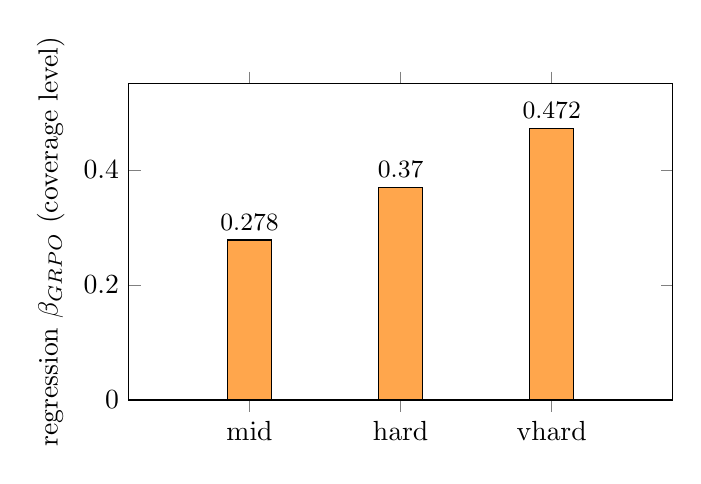
\begin{tikzpicture}
\begin{axis}[
  width=0.7\textwidth, height=5.6cm,
  ybar, bar width=16pt,
  ymin=0, ymax=0.55,
  ylabel={regression $\beta_{\text{GRPO}}$ (coverage level)},
  symbolic x coords={mid, hard, vhard},
  xtick=data,
  enlarge x limits=0.4,
  nodes near coords, nodes near coords style={font=\small},
  every node near coord/.append style={/pgf/number format/fixed,/pgf/number format/precision=3},
]
\addplot[fill=orange!70] coordinates {(mid,0.278) (hard,0.370) (vhard,0.472)};
\end{axis}
\end{tikzpicture}
\caption{Accessibility gating (Emp.~Reg.~1). As difficulty rises (headroom up,
accessibility down), regression under on-policy RL grows monotonically---usable
per-prompt signal vanishes exactly where headroom is largest, so more headroom
does not translate into more gain. Reported as a pooled empirical shape, not a
causal law.}
\label{fig:beta}
\end{figure}
